\documentclass[12pt]{article}

\usepackage[T2A]{fontenc}


\usepackage[english, russian]{babel}

\usepackage{geometry}
\geometry{a4paper, portrait, margin=0.75in}

\usepackage[normalem]{ulem}
\usepackage{fixltx2e}
\usepackage{float}
\usepackage{enumitem}
\usepackage{setspace}
\usepackage{graphicx}
\usepackage[table]{xcolor}
\usepackage{transparent}
\usepackage{bm}

\usepackage{amsmath}
% Change * to \dot
\DeclareMathSymbol{*}{\mathbin}{symbols}{"01}

\definecolor{aquamarine}{rgb}{127,255,212}
\newcolumntype{e}{>{\columncolor{yellow}}c}

\usepackage{listings}
\usepackage{color}
\def\matlab{/mnt/c/University/CAPR/MATLAB/}
\definecolor{MLgreen}{RGB}{28,172,0} % color values Red, Green, Blue
\definecolor{MLlilas}{RGB}{170,55,241}
\lstset{language=Matlab,%
    %basicstyle=\color{red},
    basicstyle=\footnotesize\fontfamily{cmr},
    breaklines=true,%
    morekeywords={matlab2tikz},
    keywordstyle=\color{blue},%
    morekeywords=[2]{1}, keywordstyle=[2]{\color{black}},
    identifierstyle=\color{black},%
    stringstyle=\color{MLlilas},
    commentstyle=\color{MLgreen},%
    showstringspaces=false,%without this there will be a symbol in the places where there is a space
    numbers=left,%
    numberstyle={\tiny \color{black}},% size of the numbers
    numbersep=9pt, % this defines how far the numbers are from the text
    emph=[1]{for,end,break},emphstyle=[1]\color{red}, %some words to emphasise
    %emph=[2]{word1,word2}, emphstyle=[2]{style},
    frame = single,
}

\usepackage{hyperref}
\hypersetup{
    colorlinks,
    citecolor=black,
    filecolor=black,
    linkcolor=black,
    urlcolor=black
}

\begin{document}

\begin{titlepage}
    \begingroup
\fontsize{12pt}{14pt}\selectfont

\begin{center}

    Санкт-Петербургский политехнический университет имени Петра великого\\
    Институт компьютерных наук и кибербезопасности\\
    Высшая школа компьютерных технологий и информационных систем\\

    \vspace{\fill}

    \onehalfspacing
    \textbf{\huge Лабораторная работа \textnumero 12}\\
    \medbreak
    Дисциплина:\textbf{Телекоммуникационные технологии}\\
    Тема: Узкополосный FM-трансивер\textbf{}\\
    \vspace{1.5cm}
\end{center}


\begin{flushright}
    \doublespacing
    Выполнил студент гр. 5130901{\textbackslash}10101 \underline{\hspace{7em}} Писарик М.В.\\
    \smallskip
    Принял преподаватель \uline{\hspace{7em}}Богач Н.В. \\
    \smallskip
    "\uline{\hspace{1.5em}}" \uline{\hspace{5em}} 2024 г.\\
\end{flushright}

\vspace{\fill}

\begin{center}
    Санкт-Петербург\\
    2024 г.\\
\end{center}

\singlespacing

\pagebreak

\endgroup


\end{titlepage}



\section*{Задание}
Сгенерировать и принимать узкополосный FM-сигнал (NBFM). Вместо использования какого-либо реального оборудования для передачи сигнал отправляется через сокет из секции передачи в секцию приема. Единственное задействованное аппаратное обеспечение — это вход микрофона и выход динамика компьютера. В случае компьютера Raspberry Pi, у которого нет микрофонного входа, представлены три альтернативы.
\section*{НБФМ-приемник}
\subsection*{Блок-схема}
Используя gnuradio-companion (GRC) и следующие описания блоков, я построил блок-схему для раздела приемника:

\begin{figure}[H]
    \centering
    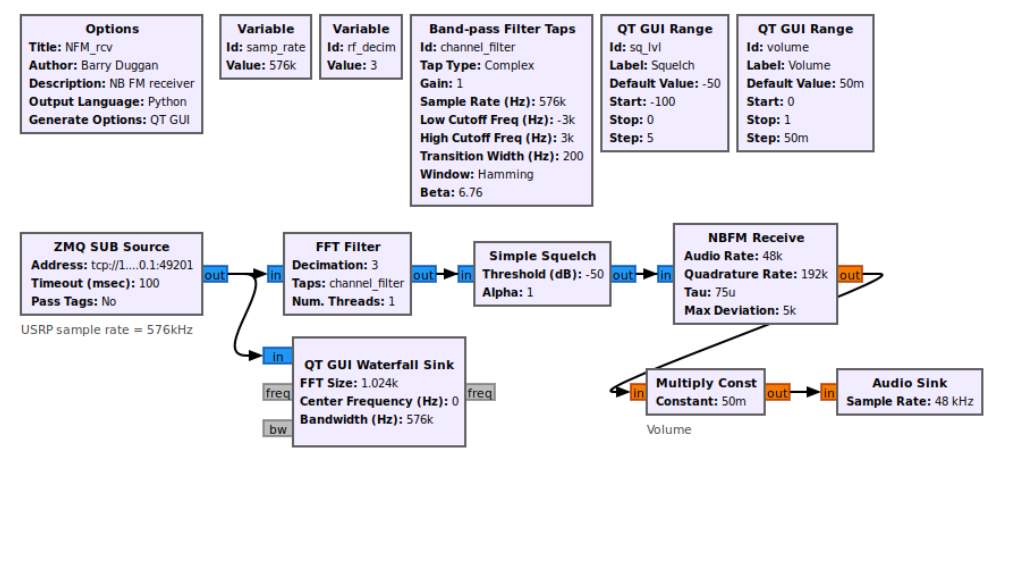
\includegraphics[width=1\textwidth]{pictures/1.png}
    \caption{НБФМ-приемник}
\end{figure}
Файл GR, как и другие файлы, используемые в этом моделировании, являются частью пакета в \href{https://github.com/duggabe/gr-control}{https://github.com/duggabe/gr-control}. Яклонировал этот репозиторий, для того, что бы создать полный приемопередатчик NBFM, использующий Pluto SDR.

\section*{Описания блоков} 
\begin{flushleft}   
    

\begin{itemize}
    
    \item Данные принимаются от передатчика через ZMQ\_SUB\_Source с частотой дискретизации 576 кГц. ПРИМЕЧАНИЕ. Измените адрес ZMQ\_SUB\_Source на tcp://127.0.0.1:49203, чтобы он мог подключаться к передатчику.
    \item Он фильтруется до полосы пропускания 6 кГц и прореживается (уменьшается) в 3 раза с помощью FFT\_Filter , что дает выходную частоту дискретизации 192 кГц.
    Simple\_Squelch отключает звук , когда уровень входного сигнала меньше уровня шумоподавления.
    \item Блок NBFM\_Receive демодулирует входной сигнал и создает выходную частоту дискретизации 48 кГц, которая соответствует желаемой частоте звука.
    \item Блок Multiply\_Const реализует регулятор громкости.
    \item Выход динамика определяется блоком Audio\_Sink.
    \begin{itemize}
        \item Имя устройства: для большинства динамиков (или разъемов для наушников), встроенных в компьютер, имя устройства можно оставить пустым; в других случаях см. Audio\_SinkDevice\_Name.
        \item Разрешено блокировать: Да
    \end{itemize}

        
  \end{itemize}
\end{flushleft}
\section*{Раздел тестового приемника} 
Без передатчика тестировать особо нечего, но вы можете сгенерировать и запустить блок-график. Через несколько секунд откроется окно графического интерфейса с элементами управления громкостью и шумоподавлением, а также отображением водопадного спектра. Обратите внимание, что водопад не будет работать, поскольку нет входных данных. Чтобы аккуратно завершить процесс, нажмите «X» в верхнем углу графического интерфейса, а не используйте Control-C.

\section*{НБФМ-передатчик} 

\section*{Блок-схема} 

Используя gnuradio-companion (GRC) и следующие описания блоков, я построил блок-схему для раздела передатчика:

\begin{figure}[H]
    \centering
    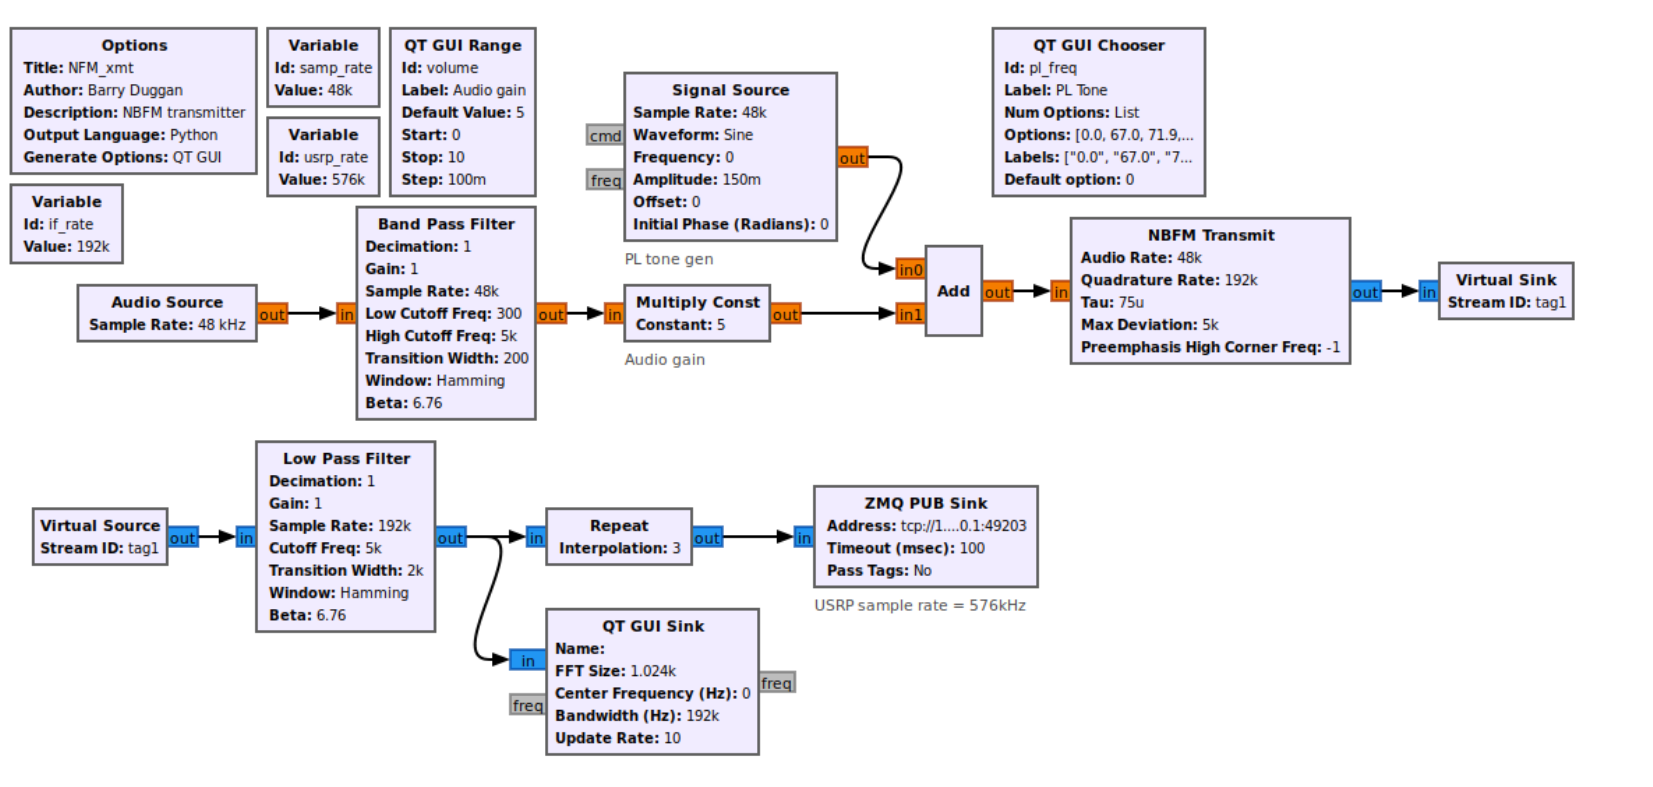
\includegraphics[width=1\textwidth]{pictures/2.png}
    \caption{НБФМ-передатчик}
\end{figure}
\section*{Описания блоков} 
\begin{flushleft}   


\begin{itemize}
    
        \item Вход микрофона определяется блоком Audio\_Source . Параметры:
        \begin{itemize}\item Частота дискретизации установлена на 48 кГЦ
        \item Имя устройства: для большинства разъемов микрофона, встроенных в компьютер, имя устройства можно оставить пустым; в других случаях см. Audio\_Source\#Device\_Name.
        \item Разрешено блокировать: Нет
\end{itemize}

    \item Звук фильтруется в диапазоне от 300 до 5000 Гц с помощью Band\_Pass\_Filter .
    \item Блок Multiply\_Const реализует элемент управления Audio Gain.
    \item Большинство репитеров используют тональный сигнал для запуска передатчика.
    \begin {itemize}
        \item Тон PL (частная линия) можно выбрать с помощью QT\_GUI\_Chooser . Использование значения 0,0 отключает PL.
        \item Signal\_Source генерирует тон PL.
    \end{itemize}
    \item Аудиосигнал плюс тон PL подаются в блок NBFM\_Transmit . Выходная частота дискретизации составляет 192 кГц.
    \item Low\_Pass\_Filter ограничивает сигнал до 5 кГц .
    \item Блок повтора интерполирует (умножает) частоту дискретизации на 3, давая выходную частоту 576 кГц.
    \item Сигнал передачи подается на ZMQ\_PUB\_Sink с адресом `tcp://127.0.0.1:49203`, соответствующим порту получателя. 
  \end{itemize}
\end{flushleft}
\section*{Тестирование} 
Запустив передачтик и приемник,  я получил гафик частоты передаваемого сигнала(моего голоса), это можно увидеть на приложенном снимке экрана. Уровень модуляции можно регулировать с помощью регулятора усиления передачи.

\begin{figure}[H]
    \centering
    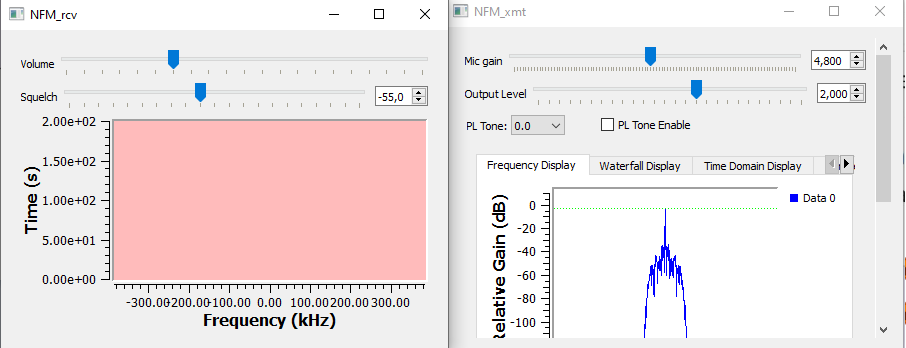
\includegraphics[width=1\textwidth]{pictures/3.png}
    \caption{Работа НБФМ-приемника и НБФМ-передатчика}
\end{figure}

\pagebreak

\end{document}
